\chapter{Chapter 3:Méthodologie}

Notre recherche, axée sur l’efficacité de la détection de modules actifs dans des réseaux biologiques, adopte une approche innovante basée sur des données multivues. Afin de rester en continuité avec les recherches précédentes, nous envisageons d'intégrer cette approche multivue au sein du framework AMINE, reconnu pour ses performances supérieures dans l'analyse de données univues avec des graphes pondérés au niveau des nœuds. Pour cela, nous établirons un cadre conceptuel qui intègre la construction de différentes vues du graphe et d'autres règles sur le processus d'intégration d'embeddings multivues dans AMINE.

\section{Cadre conceptuel}

Pour atteindre nos objectifs, nous avons défini un cadre conceptuel articulé autour de plusieurs processus clés. Initialement, nous construisons deux vues distinctes à partir d'un graphe de données pondéré, adapté au framework AMINE. Cette approche vise à assurer une continuité avec les recherches précédentes utilisant AMINE, qui a démontré d'excellents résultats dans la détection de modules actifs. La première vue sera influencée par la topologie structurelle du graphe, tandis que la seconde se concentrera sur les poids des nœuds, reflétant les p-values des protéines dans le graphe.

L'étape suivante consiste à unifier ces deux vues dans un espace vectoriel commun. Cette fusion est cruciale pour créer une représentation complète et intégrée des données. Après avoir établi cet espace vectoriel unifié, nous appliquerons l'algorithme glouton d'AMINE sur l'embedding résultant. Cependant, avant d'appliquer cet algorithme, il est essentiel de définir des métriques de similarité adaptées à ce nouvel embedding. Ces métriques seront déterminantes pour évaluer la pertinence et l'efficacité de notre approche multivue dans la détection de modules actifs.

Notre démarche implique également une analyse approfondie des caractéristiques intrinsèques des données biologiques (au niveau de la validation des données ) , en tenant compte de la variabilité et de la complexité des interactions génétiques. En intégrant ces aspects, nous visons à améliorer la précision de la détection des modules actifs.

Nous illustrons notre cadre conceptuel avec la Figure \ref{fig:cadre_conceptuel}.

\begin{figure}[h]
\centering
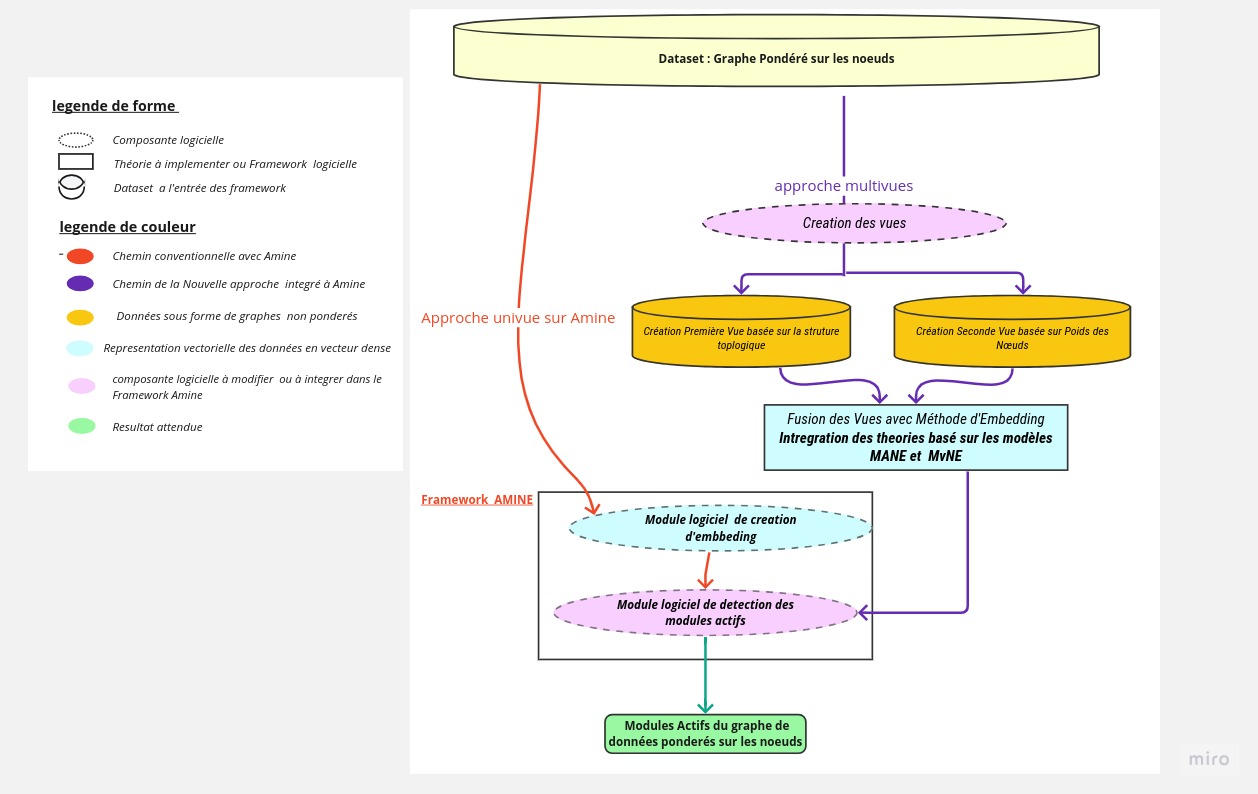
\includegraphics[width=1\textwidth]{Pictures/cadre_conceptuel.jpg}
\captionsetup{justification=centering}
\caption{Illustration de notre cadre conceptuel via l'approche multivues}
\label{fig:cadre_conceptuel}
\end{figure}


\section{Conception du modèle}

\subsection{Modèles de Construction de la Première Vue}
La construction des vues est un élément central de notre recherche. La première vue, en particulier, joue un rôle crucial dans l'analyse des données. Cette vue est conçue comme une réplique fidèle du graphe d'origine, mais sans pondération au niveau des nœuds. En adoptant cette méthode, nous préservons intégralement la structure topologique du graphe, ce qui nous permet de capturer et d'analyser les relations et les connexions intrinsèques entre les différents nœuds. Cette préservation de la structure topologique est essentielle pour deux raisons. Premièrement, elle permet une interprétation plus directe et intuitive des relations entre les nœuds, car chaque lien ou connexion dans le graphe reflète une interaction ou une association réelle, non influencée par des poids. Deuxièmement, en conservant la structure originale, elle nous permet de fidéliser les propriétés de connectivité des protéines pour une activité biologique.


\subsection{Modèles de Construction de la Deuxième Vue}
Pour la deuxième vue, nous avons élaboré quatre modèles de construction distincts, chacun proposant deux sous-variantes basées sur des règles de filtrage spécifiques. Les nœuds qui ne respectent pas ces règles seront traités soit comme des singletons (première variante) soit retirés complètement (seconde variante)
    \begin{enumerate}
        \item  \textbf{Modèle Construction 1} : Filtrage des composantes connexes du graphe où les relations sont établies uniquement avec les nœuds ayant une p-value inférieure ou égale à 0.05.
            \begin{itemize}
                \item  Sous-Variante 1 :Les autres nœuds non connectés sont considérés comme des singletons.
                \item Sous-Variante 2 : Ces nœuds sont retirés.
            \end{itemize}
        \item \textbf{Modèle Construction 2 }:Filtrage de tous les nœuds avec une p-value inférieure à 0.05 pour créer une composante connexe complète avec cet ensemble de noeuds de p\_value inferieur ou egale à 0.05 .
            \begin{itemize}
              \item Sous-Variante 1 : Les nœuds avec une p-value supérieure à 0.05 deviennent des singletons.
               \item Sous-Variante 2 : Ces nœuds sont retirés.
            \end{itemize}
        \item \textbf{Modèle Construction 3}  : La seconde vue a la même structure topologique que la première, mais avec des arêtes supplémentaires entre les nœuds de p-value inférieure à 0.05 pour former un sous-graphe complet.
            \begin{itemize}
                \item Sous-Variante 1 : Traitement des nœuds singletons existants.
                \item Sous-Variante 2 : dans cette construction la sous variante n'exite pas car dans le graphe d'origine nous n'avons pas de noeud singletions, lors de la construction du graphe nous veillons a ce que toutes les composance connexe soient liés par au moins une arrete .
            \end{itemize}
      \item \textbf{Modèle Construction 4 }: Construction d'un graphe en ajoutant des arêtes entre les nœuds dont la différence de "ZScores" est inférieure ou égale à 0.4.
        \begin{itemize}
            \item Sous-Variante 1 : Les nœuds non connectés sont considérés comme des singletons.
          \item  Sous-Variante 2 : Ces nœuds sont retirés 
        \end{itemize}
     
    \end{enumerate}

\subsection{choix du Modèles de theorie d'unifictaion d'embbedding }
Le choix entre ces variantes influencera la méthode d'intégration unifiée, en tenant compte des capacités des frameworks comme MANE (Multi-View Collaborative Network Embedding), adapté aux vues complètes, et MvMe (Multi-view Neighbourhood Embedding), plus efficace pour les vues incomplètes. Des tests préliminaires seront réalisés pour évaluer l'efficacité de ces différentes approches afin d'adopter un modèle final.

La sélection du modèle optimal pour la deuxième vue est essentielle, car elle influence directement la qualité des informations utilisées dans notre analyse finale. Chaque modèle d'intergartion unifie sera   seront évalués sous les deux variantes de la secondes vues . L'objectif est de déterminer la combinaison la plus efficace pour la détection de modules actifs, en se basant sur des critères tels que la précision, la robustesse et la pertinence biologique, ainsi que la métrique de similarité de validation sur l'embedding unifié. En appliquant ces critères d'évaluation rigoureux, nous nous assurons que le modèle choisi offre non seulement une représentation précise des données biologiques, mais est également robuste et adapté à divers contextes d'analyse.
 
\subsection{Critères d'Évaluation}

Pour évaluer et valider nos modèles dans le but d'assurer leur efficacié et leur fiabilité , nous avons élaboré trois critères principaux, chacun ciblant un aspect différent de la performance du modèle :

\begin{enumerate}

    \item \textbf{la Métrique Précision :}
    
        La capacité du modèle à identifier correctement les modules actifs est mesurée par le score F1. Ce critère évalue l'équilibre entre la précision (proportion de vrais positifs parmi les identifications) et le rappel (proportion de vrais positifs parmi les cas réels). La formule du score F1 est la suivante :
            \begin{equation}
            \text{F1 Score} = 2 \times \frac{\text{Précision} \times \text{Rappel}}{\text{Précision} + \text{Rappel}}
            \end{equation}
            Où :
            \begin{itemize}
                \item La précision est calculée comme \(\frac{TP}{TP + FP}\)
                 \item  Le rappel est calculé comme \(\frac{TP}{TP + FN}\)
                 \item \(TP\) représente le nombre de vrais positifs (Vrai positives).
                 \item  \(FP\) représente le nombre de faux positifs (Faux positives).
                 \item \(FN\) représente le nombre de faux négatifs (Faux negatives).
            \end{itemize}
            
    \item \textbf{Métrique de similarité:} 
        Nous avons défini trois métriques dans l'espace unifié pour évaluer la similarité des représentations vectorielles des nœuds. Ces métriques comprennent la similarité cosinus, la distance euclidienne, et la similarité de Pearson. 
        \begin{itemize}
           \item \textbf{\textit{La Similarité de Pearson :}}
                La similarité de Pearson (ou corrélation de Pearson) mesure la corrélation linéaire entre deux variables aléatoires. La formule pour calculer la corrélation de Pearson entre deux vecteurs \(X\) et \(Y\) est :
                \begin{equation}
                     r = \frac{\sum_{i=1}^{n} (X_i - \bar{X})(Y_i - \bar{Y})}{\sqrt{\sum_{i=1}^{n} (X_i - \bar{X})^2} \sqrt{\sum_{i=1}^{n} (Y_i - \bar{Y})^2}}
                \end{equation}
                où \(\bar{X}\) et \(\bar{Y}\) sont les moyennes des vecteurs \(X\) et \(Y\) respectivement. La valeur de \(r\) se situe entre -1 et 1.
                
           \item \textbf{\textit{La Similarité Cosinus :}}
           
                La similarité cosinus mesure l'angle entre deux vecteurs dans un espace vectoriel. Elle est calculée comme le produit scalaire des vecteurs normalisé par le produit de leurs normes. La formule est :
                \begin{equation}
                       \text{similarity\_cosine} = \frac{X \cdot Y}{\|X\| \|Y\|}
                \end{equation}
             
                où \(X \cdot Y\) est le produit scalaire des vecteurs \(X\) et \(Y\), et \(\|X\|\) et \(\|Y\|\) sont les normes de \(X\) et \(Y\).
                
            \item\textbf{\textit{La Similarité Euclidienne :}}
            
                La similarité euclidienne (ou distance euclidienne normalisée) est basée sur la distance euclidienne entre deux points. Si \(D\) est la distance euclidienne entre deux vecteurs \(X\) et \(Y\), la similarité \(S\) est calculée comme :
                \begin{equation}
                    \text{Similarity\_euclidienne} = \frac{1}{1 + D}
                \end{equation}
                  où \(D\) est la distance euclidienne, calculée comme :
                  \[ D = \sqrt{\sum_{i=1}^{n} (X_i - Y_i)^2} \]
         \end{itemize}
        
    Chacune de ces métriques de similarité apporte une perspective différente sur la manière dont les nœuds ou les modules sont liés ou distants les uns des autres dans l'espace vectoriel.
    
   \item \textbf {Robustesse} (Test sur Ensemble de Données Artificiel):
        
    La stabilité du modèle est testée sur un ensemble de données artificiel comprenant 1000 graphes. Ce critère évalue la capacité du modèle à maintenir une performance constante malgré les variations dans les données d'entrée, assurant ainsi sa robustesse et sa fiabilité.
\end{enumerate}

Nous pouvons illustrons notre modele conceptuel avec la Figure \ref{fig:Modele_conceptuel}.

\begin{figure}[h]
\centering
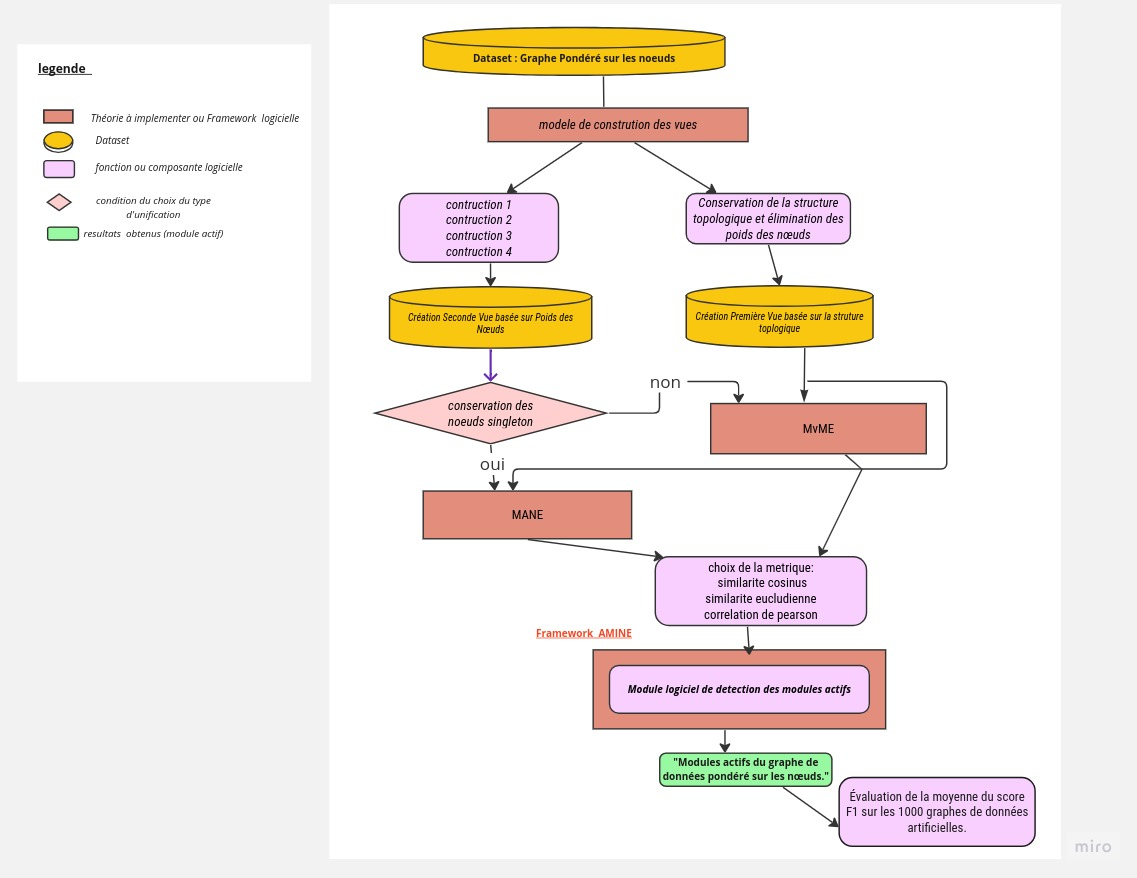
\includegraphics[width=0.85\textwidth]{Pictures/modele_conceptuel.jpg}
\captionsetup{justification=centering}
\caption{Illustration de notre modele conceptuel}
\label{fig:Modele_conceptuel}
\end{figure}


\section{ Collecte de données:}

Dans le cadre de notre étude, nous avons opté pour la création de données artificielles afin de simuler des réseaux biologiques complexes. Cette méthode nous permet de contrôler précisément les paramètres du réseau, ce qui est crucial pour tester l'efficacité de notre modèle de détection de modules actifs. Après avoir validé le modèle sur ces données artificielles, nous l'appliquerons sur des données réelles, celles générées dans l'article de Chiou et al. Le modèle AMINE a également été évalué sur ces données.


\subsection{Description de l'Algorithme de Génération de Données } 

Cet algorithme génère des données en simulant des réseaux biologiques complexes à l'aide de graphes sans échelle. Il s'appuie sur une version améliorée de la méthode de Barabási-Albert, idéale pour modéliser des réseaux où la distribution des degrés des nœuds suit une loi de puissance. En plus d'intégrer la méthode de Barabási-Albert, l'algorithme comprend trois fonctions principales qui sont  utiles dans la construction des clusters  :

\begin{enumerate}
    \item \textbf{neighbors} :
    son Rôle est de  détermine le nombre de voisins d'un nœud spécifique à une distance d'orde \(k\).  Partant d'un nœud initial (\(start\)), elle explore et compte les voisins jusqu'à atteindre le niveau \(k\), offrant ainsi une vue sur la connectivité locale du nœud dans le graphe.

    \item \textbf{knbrs} :
     Cette fonction identifie tous les voisins d'un nœud à un niveau \(k\).
     Similaire à \textit{neighbors\_order}, elle retourne un ensemble des voisins jusqu'au niveau \(k\), permettant de comprendre les interactions potentielles d'un nœud donné.

    \item \textbf{get\_seeds} : Cette fonction sélectionne des nœuds initiaux pour la création de modules dans le graphe. et veuille a ce que les  nœuds  soient suffisamment éloignés les uns des autres (\(min\_distance\)), assurant ainsi une distribution équilibrée et non chevauchante des modules dans le graphe.
  
\end{enumerate}

Chaque sous-fonction joue un rôle clé dans l'élaboration d'un graphe complexe et structuré, reflétant les propriétés des réseaux biologiques. \textit{neighbors\_order} et \textit{knbrs} sont cruciales pour analyser la structure locale des nœuds, tandis que \textit{get\_seeds} est essentielle pour initier la formation de modules distincts au sein du graphe.

\begin{figure}[h]
\centering
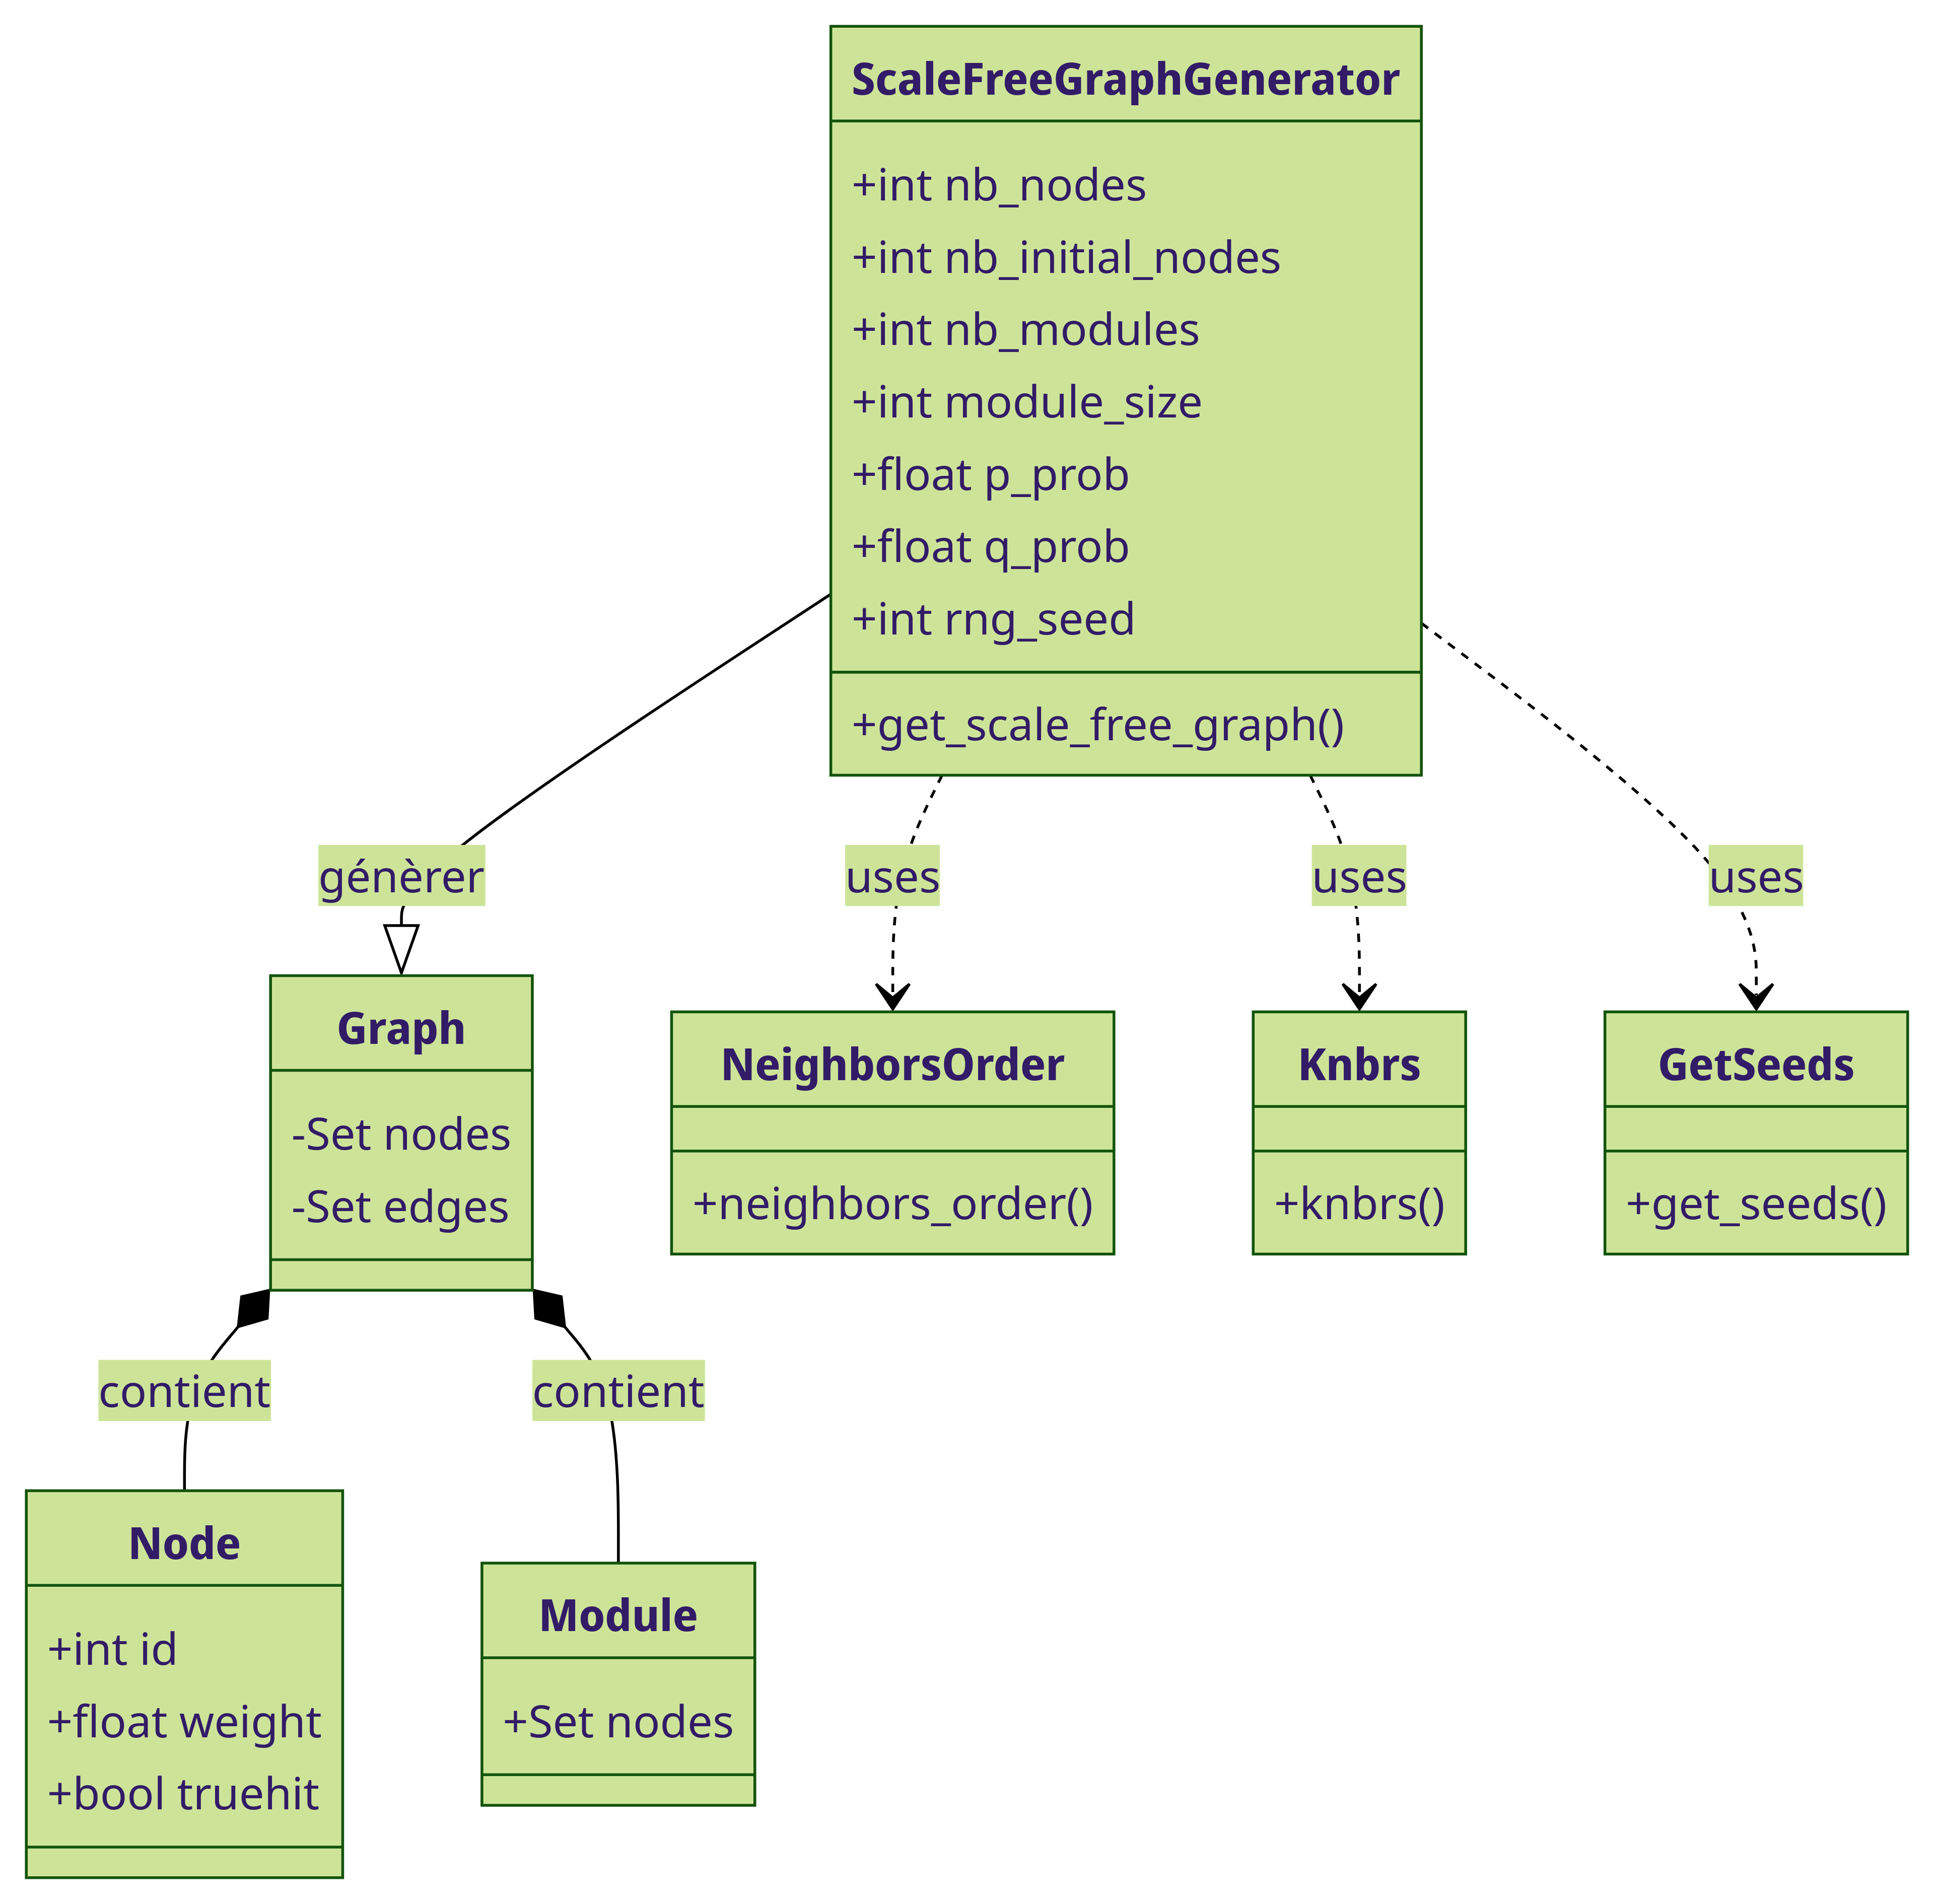
\includegraphics[width=0.50\textwidth]{Pictures/classe_diagramDonnee.png}
\captionsetup{justification=centering}
\caption{Illustration en digaramme classe de la desciption de l"agorithme qui genere les données artificielles }
\label{fig:classe_Diagramme}
\end{figure}

\subsection{ Génération de la structure topologique du graphe}

la structure topologique du  reseaux de données  est   basé sur le modèle de Barabási-Albert étendu, permettant la création de graphes libres d'échelle avec la propriete fondamentale de l'attachement préférentiel (Les nouveaus noeuds  ont tendance à se connecter à des nœuds déjà bien connecté). Les paramètres clés de ce modele  sont :

\begin{enumerate}
    \item Nœuds Initiaux ( \textit{nb\_initial\_nodes =3}) : 
     Les nœuds initiaux forment le noyau de départ du graphe. Ils sont essentiels pour commencer le processus de croissance du réseau selon la méthode de Barabási-Albert. Le nombre de nœuds initiaux influence la structure initiale du réseau. Un petit nombre de nœuds initiaux peut conduire à un réseau plus centralisé autour de ces nœuds, tandis qu'un plus grand nombre peut favoriser une structure plus distribuée. Le choix du nombre de nœuds initiaux doit refléter l'objectif de la simulation. Pour un réseau biologique, il est souvent souhaitable de commencer avec un petit nombre de nœuds initiaux pour simuler le développement naturel d'un réseau biologique à partir de quelques éléments clés.
    
    \item Probabilités (\textit{p\_prob}) et (\textit{q\_prob}) : 
      la probabilité (\textit{p\_prob}=0.09): Contrôle l'ajout de nouvelles arêtes entre les nœuds existants. Un (\textit{p\_prob}) élevé favorise la création de nouvelles connexions.  et la probabilité  (\textit{q\_prob}=0.7): Gère la réorganisation des arêtes existantes. Un (\textit{q\_prob}) élevé permet une plus grande dynamique dans la structure du réseau.
      pour assure un équilibre entre la croissance et la reorganistaion du réseau la somme de probabilité doit soumise a  la contrainte suivante  \( (\textit{p\_prob})+ (\textit{q\_prob}) < 1 \),

\end{enumerate}
Après avoir construit la structure topologique du graphe basée sur le modèle de Barabási-Albert, nous veillerons à ne pas laisser de composantes connexes disjointes. Le principe est simple,il s'agira de créer un lien aléatoire entre les composantes connexes.

\subsection{Génération des Modules dans le Graphe }

La formation des modules dans le réseau est une étape cruciale, simulant la création de groupes de gènes ou de protéines fonctionnellement liés. Des nœuds "graines" sont sélectionnés en fonction de leur degré de connectivité et de leur distance relative, assurant une répartition équilibrée des modules dans le graphe. Autour de chaque graine, un module est formé en intégrant des nœuds voisins, choisis selon un processus aléatoire pondéré par la distance dans le graphe. La taille de chaque module est contrôlée par le paramètre `module\_size`. Par exemple, si une graine est sélectionnée, les nœuds à une distance de 1 ou 2 pas sont progressivement inclus dans le module, en fonction de leur probabilité de connexion.

\subsection{ Attribution des Poids (p\_value) aux Nœuds}

Enfin, des poids sont attribués à chaque nœud du graphe pour simuler des caractéristiques biologiques spécifiques. Les nœuds hors modules reçoivent des poids selon une distribution uniforme [0,1], tandis que ceux au sein des modules suivent une distribution normale tronquée. Cette distribution est choisie pour refléter une concentration élevée de caractéristiques biologiquement significatives dans les modules, comme on pourrait s'y attendre dans des groupes de gènes ou de protéines actifs. Les poids des nœuds dans les modules sont donc générés selon la formule :
    \begin{equation}
         P(\text{p\_value}) = \text{TruncNorm}(\mu, \sigma, a, b) \
    \end{equation}
    
    où \(\mu = 0\), \(\sigma = 0.05\), et les bornes \(a\) et \(b\) sont ajustées pour maintenir les poids entre 0 et 1.
    
\begin{figure}[h]
\centering
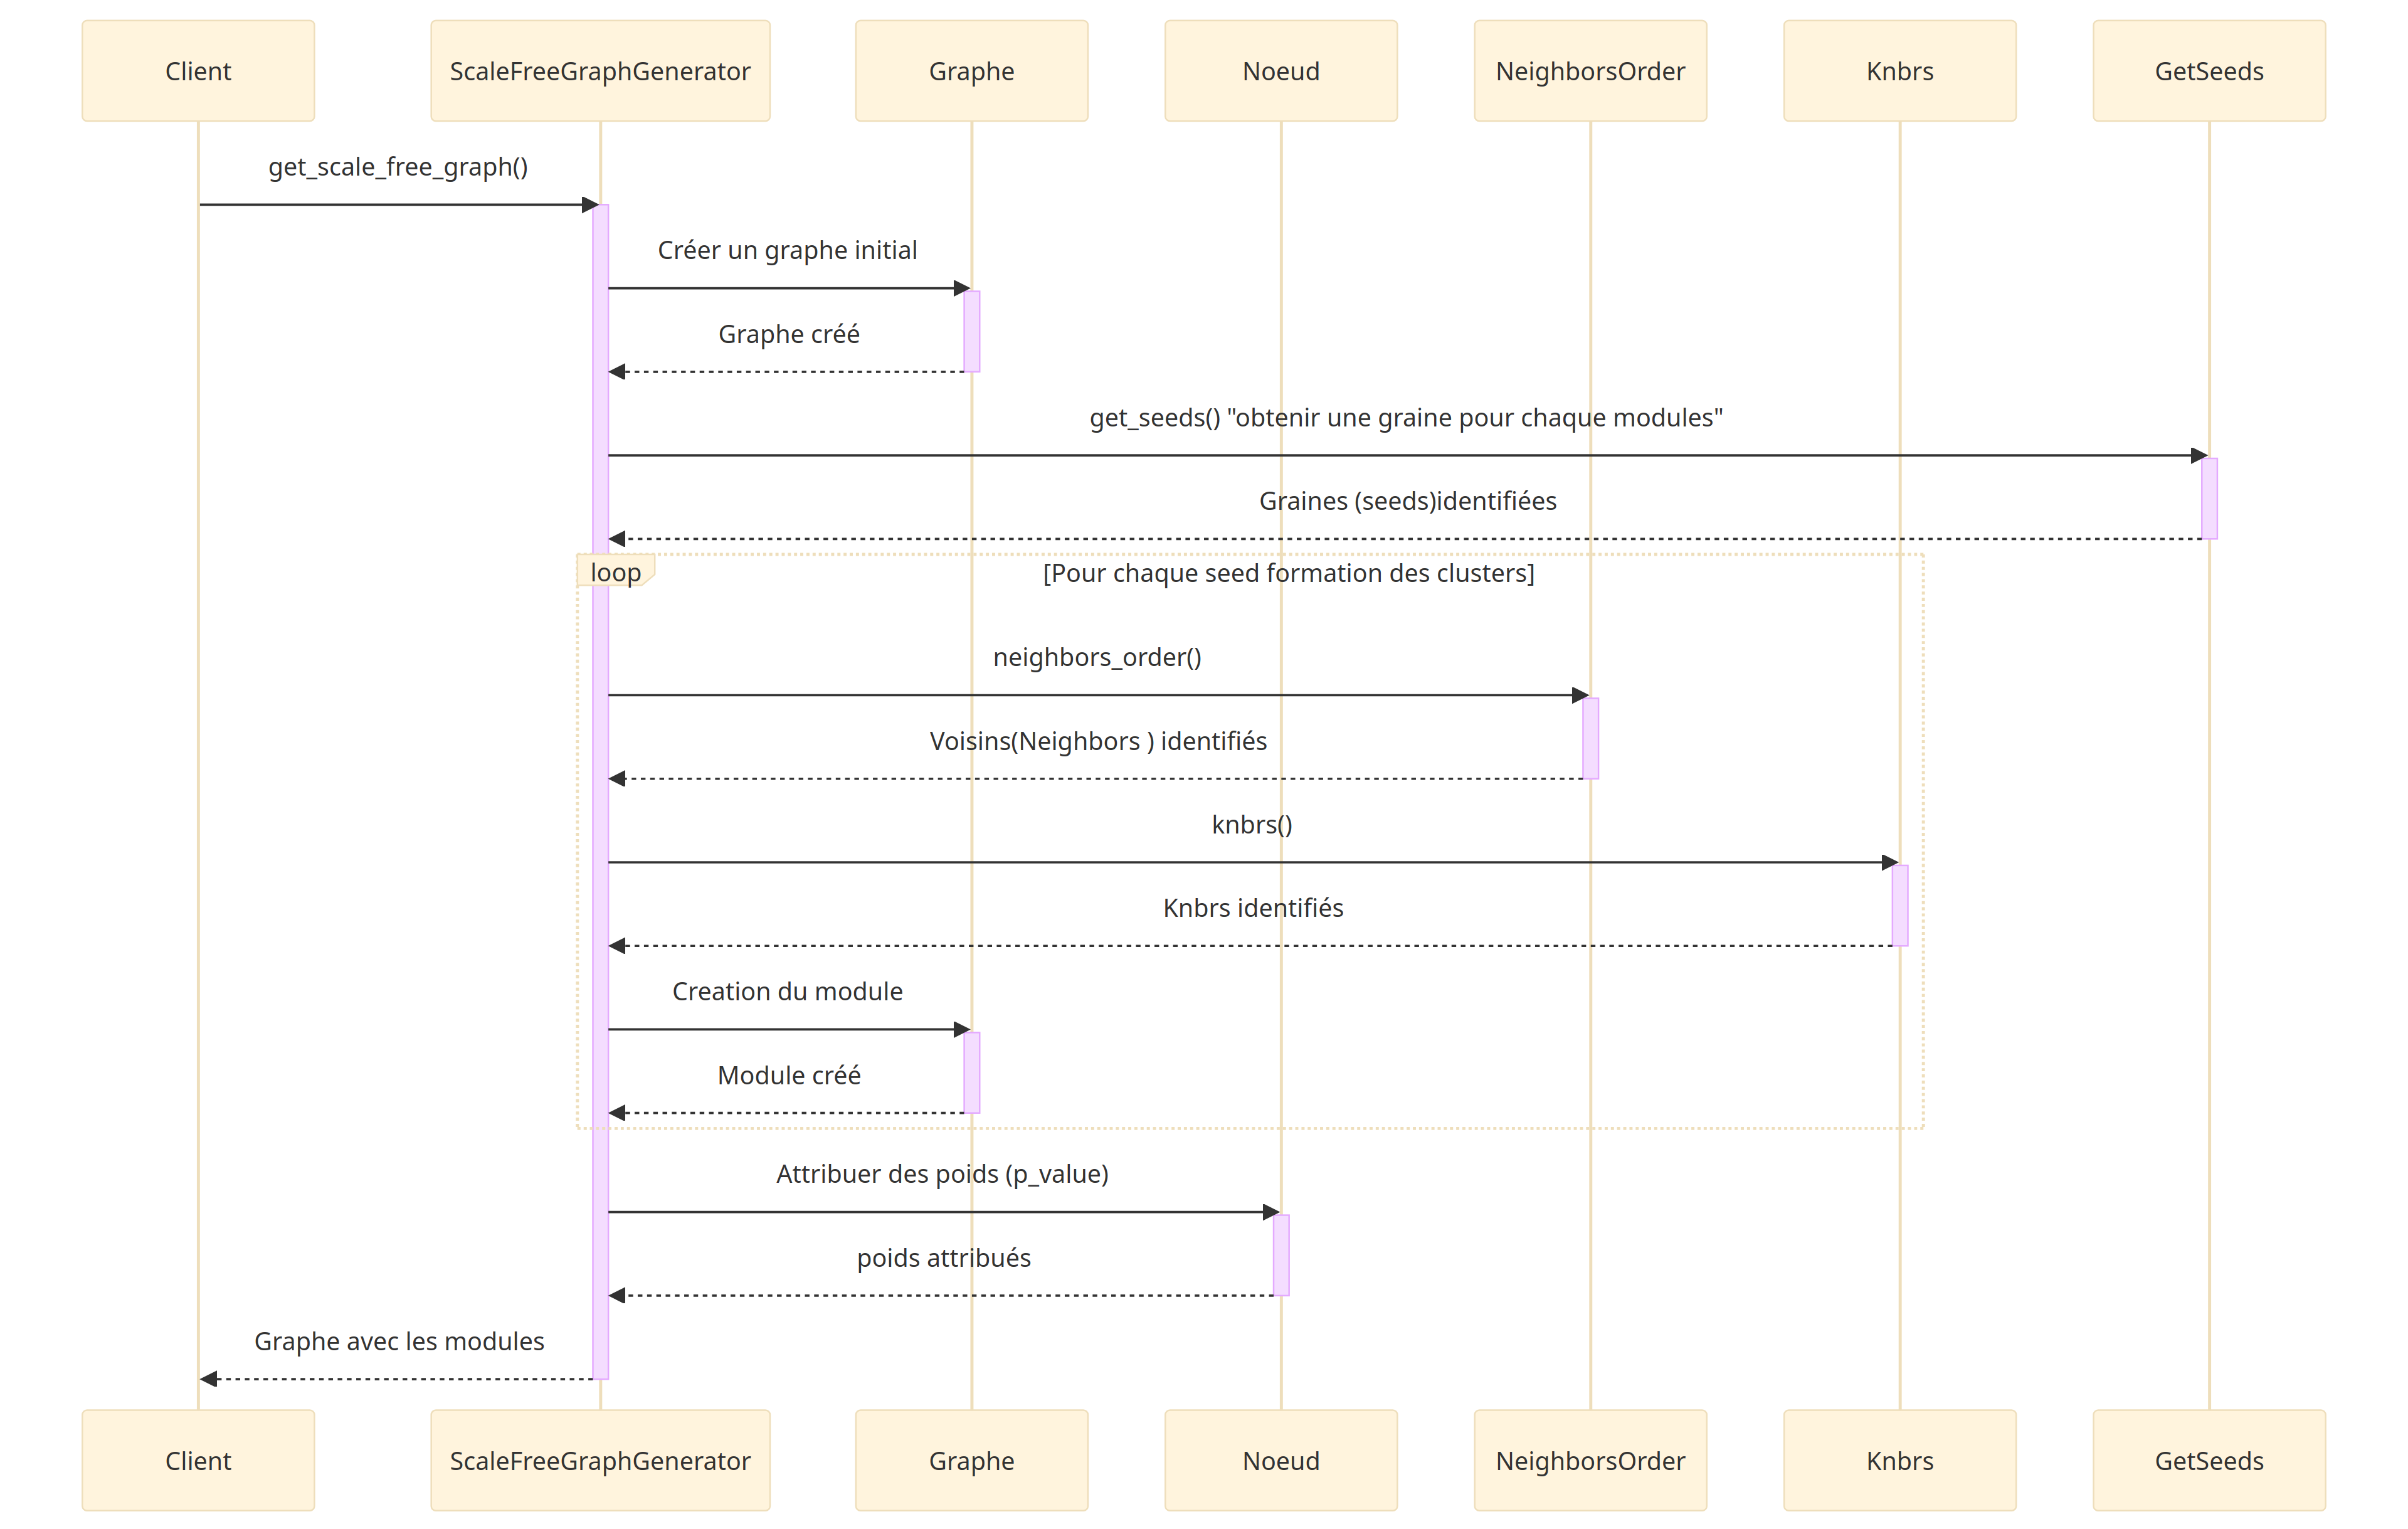
\includegraphics[width=1\textwidth]{Pictures/sequence_diagramme.png}
\captionsetup{justification=centering}
\caption{Illustration la gereration des  données artificielles }
\label{fig:sequence_Diagramme}
\end{figure}

La méthodologie proposée offre une nouvelle perspective pour l'analyse des interactions complexes au sein des réseaux biologiques en intégrant le concept de données multivues et en appliquant des critères d'évaluation rigoureux, nous visons à améliorer la précision et la robustesse de la détection des modules actifs, un aspect crucial pour la compréhension des mécanismes biologiques sous-jacents

